%-------------------------------------------------------------------------------
% This file is for the Glance-GitLab supporting note about the ATLAS publication procedure
% \pdfinclusioncopyfonts=1
% This command may be needed in order to get \ell in PDF plots to appear. Found in
% https://tex.stackexchange.com/questions/322010/pdflatex-glyph-undefined-symbols-disappear-from-included-pdf
%-------------------------------------------------------------------------------
% Specify where ATLAS LaTeX style files can be found.
\newcommand*{\ATLASLATEXPATH}{latex/}
% Use this variant if the files are in a central location, e.g. $HOME/texmf.
% \newcommand*{\ATLASLATEXPATH}{}
%-------------------------------------------------------------------------------
\documentclass[NOTE, atlasdraft=true, texlive=2016, UKenglish, txfonts]{\ATLASLATEXPATH atlasdoc}
% Use txfonts while the note is in Overleaf, due to a newtx bug with this TeX Live version.
% Commonly used options:
%  atlasdraft=true|false This document is an ATLAS draft.
%  texlive=YYYY          Specify TeX Live version (2016 is default).
%  txfonts=true|false    Use txfonts rather than the default newtx
%  paper=a4|letter       Set paper size to A4 (default) or letter.

%-------------------------------------------------------------------------------
% Extra packages:
\usepackage{\ATLASLATEXPATH atlaspackage}
% Commonly used options:
%  biblatex=true|false   Use biblatex (default) or bibtex for the bibliography.
%  subfigure|subfig|subcaption  to use one of these packages for figures in figures.
%  minimal               Minimal set of packages.
%  default               Standard set of packages.
%  full                  Full set of packages.
%-------------------------------------------------------------------------------
% Style file with biblatex options for ATLAS documents.
\usepackage{\ATLASLATEXPATH atlasbiblatex}

% Package for creating list of authors and contributors to the analysis.
\usepackage{\ATLASLATEXPATH atlascontribute}

% Useful macros
\usepackage{\ATLASLATEXPATH atlasphysics}
% See doc/atlas_physics.pdf for a list of the defined symbols.
% Default options are:
%   true:  journal, misc, particle, unit, xref
%   false: BSM, heppparticle, hepprocess, hion, jetetmiss, math, process, other, texmf
% See the package for details on the options.

% Files with references for use with biblatex.
% Note that biber gives an error if it finds empty bib files.
\addbibresource{ANA-GENR-2018-01-INT1.bib}
\addbibresource{bib/ATLAS.bib}
\addbibresource{bib/CMS.bib}
\addbibresource{bib/ConfNotes.bib}
\addbibresource{bib/PubNotes.bib}

% Paths for figures - do not forget the / at the end of the directory name.
\graphicspath{{logos/}{figures/}}

% Add you own definitions here (file ANA-GENR-2018-01-INT1-defs.sty).
\usepackage{ANA-GENR-2018-01-INT1-defs}

%-------------------------------------------------------------------------------
% Generic document information
%-------------------------------------------------------------------------------

% Title, abstract and document
% Turn off some chktex warnings.
% chktex-file 1 chktex-file 8 chktex-file 46
%-------------------------------------------------------------------------------
% This file contains the title, author and abstract.
% It also contains all relevant document numbers used for an ATLAS note.
%-------------------------------------------------------------------------------

% Title
\AtlasTitle{ATLAS publications and the role of Fence and GitLab}

% Draft version:
% Should be 1.0 for the first circulation, and 2.0 for the second circulation.
% If given, adds draft version on front page, a 'DRAFT' box on top of each other page, 
% and line numbers.
% Comment or remove in final version.
\AtlasVersion{0.1}

% Abstract - % directly after { is important for correct indentation
\AtlasAbstract{%
  The ATLAS Collaboration develops and uses web systems and tools, defines methods, establishes procedures and organizes advisory groups to manage the publication processes of scientific papers, conference papers and public notes.
  The so-called Phase 0 system was implemented using the FENCE framework and is integrated into the CERN Gitlab software repository, to automatically configure workspaces where the analysis can be documented and used by the analysis team and managed by the conveners.
  Continuous integration is used to guide the authors on using the accurate format while writing papers to be submitted to scientific journals.
  The ATLAS Physics and Committees Office provide support to the researchers and facilitate each phase of a publication process, allowing authors to focus on the article contents that describe the results and discoveries of the ATLAS experiment.
}

% Author - this does not work with revtex (add it after \begin{document})
% \author{The ATLAS Collaboration}

% Authors and list of contributors to the analysis
% \AtlasAuthorContributor also adds the name to the author list
% Include package latex/atlascontribute to use this
% Use authblk package if there are multiple authors, which is included by latex/atlascontribute
% \usepackage{authblk}
% Use the following 3 lines to have all institutes on one line
\makeatletter
\renewcommand\AB@affilsepx{, \protect\Affilfont}
\makeatother
% \renewcommand\Authands{, } % avoid ``. and'' for last author
% \renewcommand\Affilfont{\itshape\small} % affiliation formatting
\AtlasAuthorContributor{Fairouz Malek}{c}{Head of Physics Office and coordinator of Phase 0, Glance--\gitlab integration. Participation to the overal design, implementation and management of the project.}
\AtlasAuthorContributor{Ian Brock}{a}{Writer and maintainer of ATLAS \LaTeX\ templates.}
\AtlasAuthorContributor{Tancredi Carli}{b}{Physics Coordinator. Participation to the design, implementation and management of part of the project, namely Phase 0.}
\AtlasAuthorContributor{Nuno Castro}{d}{\pogitlab responsible, development and maintenance.}
\AtlasAuthorContributor{Maurizio Colautti}{f}{Developer: Fence, author list and Glance \gitlab integration, AFS and CDS related matters.}
\AtlasAuthorContributor{Ana Carolina da Silva Menezes}{e}{Developer: Glance and Fence.}
\AtlasAuthorContributor{Gabriel de Oliveira da Fonseca}{e}{Developer: Glance and Fence.}
\AtlasAuthorContributor{Andreas Hoecker}{b}{Deputy Spokesperson in charge to follow PO and Glance Team tasks. Participation to the overal design, implementation and management of the project.}
\AtlasAuthorContributor{Gabriela Lemos Lucidi Pinhao}{e}{Developer/Designer: Glance, Fence, Glance \gitlab integration.}
\AtlasAuthorContributor{Carmen Maidantchik}{e}{Glance Team Supervisor.}
\AtlasAuthorContributor{Gianluca Picco}{f}{Developer: Fence, author list and Glance--\gitlab integration.}
\AtlasAuthorContributor{Marcelo Texeira Dos Santos}{e}{\pogitlab developer and maintenance.}
\affil[a]{Universität Bonn}
\affil[b]{CERN}
\affil[c]{LPSC Grenoble}
\affil[d]{LIP Lisbon}
\affil[e]{Rio de Janeiro}
\affil[f]{Udine}
% ATLAS reference code, to help ATLAS members to locate the paper
\AtlasRefCode{ANA-GENR-2018-01}

% ATLAS note number. Can be an COM, INT, PUB or CONF note
\AtlasNote{ANA-GENR-2018-01-INT1}

% Author and title for the PDF file
\hypersetup{pdftitle={ATLAS document},pdfauthor={The ATLAS Collaboration}}

%-------------------------------------------------------------------------------
% Content
%-------------------------------------------------------------------------------
\begin{document}

\maketitle

\tableofcontents

% List of contributors - print here or after the Bibliography.
\PrintAtlasContribute{0.30}
\clearpage

You can find some text snippets that can be used in papers in \texttt{template/atlas-snippets.tex}.
Some of the snippets need the \texttt{jetetmiss} option passed to \texttt{atlasphysics}.
%\subsection{\Antikt}

The \antikt algorithm with a radius parameter of $R=0.4$ is used to reconstruct jets with a four-momentum recombination scheme, using \topos as inputs. Jet energy is calibrated to the hadronic scale with the effect of \pileup removed

\subsection{\Topos}

Hadronic jets are reconstructed from calibrated three-dimensional \topos.
Clusters are constructed from calorimeter cells that are grouped together using a topological clustering algorithm.
These objects provide a three-dimensional representation of energy depositions in the calorimeter and implement a nearest-neighbour noise suppression algorithm.
The resulting \topos are classified as either electromagnetic or hadronic based on their shape, depth and energy density.
Energy corrections are then applied to the clusters in order to calibrate them to the appropriate energy scale for their classification.
These corrections are collectively referred to as \textit{local cluster weighting}, or LCW, and jets that are calibrated using this procedure are referred to as LCW jets~\cite{PERF-2012-01}.

\subsection{Grooming}

Trimming removes subjets with $\ptsubji/\ptjet < \fcut$, where \ptsubji is the transverse momentum of the $i^{\text{th}}$ subjet, and $\fcut=0.05$.
Filtering proceeds similarly, but utilises the relative masses of the subjets defined and the original jet. For at least one of the configurations tested, trimming and filtering are both able to approximately eliminate the \pileup dependence of the jet mass.

%-------------------------------------------------------------------------------
% Introduction
\section{Introduction}
\label{sec:intro}
Will be briefly presented in this document the workflow to create an ATLAS publication together with some very important tool that are very helpful to this process like Glance/Fence and Gitlab.
%-------------------------------------------------------------------------------

%-------------------------------------------------------------------------------
% Overview of PO-GitLab
\section{Physics Office Gitlab project}
\label{sec:pogitlab}

The Physics Office GitLab project aims to simplify the ATLAS documents (papers, CONF-Notes, internal notes...) creation, editing and publication process by using the tools provided by the CERN GitLab system. The usual publication workflow consisted on a heavy e-mail communication between ATLAS editors and Physics Office in order to ensure that ATLAS rules were beeing followed before being able to submit the desired paper to arXiv or to the journal of choice. This approach lead, usually, to modifications done in different sides (Officers and editors) not properly implemented by the other side which slows down the process due to small details which with a different approach would be easily fixeable.

There are three main areas modified by the PO-GitLab approach with the goal of simplifying this process. These areas are the automatic creation of the document GitLab projects (git repositories in a centralized way), the real-time check by the GitLab Continuous Integration (CI) tools of the documents being written and the automatic processing of the document to ensure a smooth publication process. These areas are descrived in detail in this section.

\subsection{Automatic document creation}
First, a centralized area controlled by ATLAS Physics Office needs to be dessigned. The control is key in order to allow Physics Office to maintain quality controls over the document being accepted for publication. The ATLAS Physics Office GitLab group (Described in \Sect{\ref{sec:pogitlab-group}}) has been created. This GitLab group (a set of users, subgroups and projects) hosts the git repositories of ATLAS Physics Office tools as well as subgroups, one for each physics group as defined in Glance.

Since there is a centralized and standardize place to host and maintain the document repositories, these are created automatically for each analysis group once they are created in Glance in the Analysis interface. This means that the creation of configuration of the repositories holding the document is done without any input from the editor's side allowing for a quick process.

\subsection{Real-time check with GitLab's CI}
GitLab CI tools are dessigned to execute a set of automatic tasks everytime a new modification is introduced in the document (i.e. a new commit is pushed to the document repository). These tasks can be as complicated as needed within the limits of the system. The approach from Physics Office was to develop a package which is able to run different jobs on a given document checking different aspecs. This is the \texttt{pogitlab} python package~\cite{pogitlab-repo}

GitLab's CI works in Pipelines; each a time a new commit is pushed to the repository a pipeline is triggered. A pipeline is a set of jobs grouped in stages. All the jobs in the same stage are run in parallel while each stage is only executed once the previous one has finished. The real-time checks are run in most of the branches of the project, lets call them \epipes. The \epipes, showing an example in \Fig{\ref{fig:edit-pipe}} consist in the following set of stages:

\begin{itemize}
  \item \textbf{Preparation:} It consist of only one job which checks that the current version of the \texttt{pogitlab} package.
  \item \textbf{Technical checks:} This stage includes checks related to \LaTeX\:
  \begin{itemize}
    \item \textit{Figures exist:} check if all figures used throughout the document are present in the repository or if anyone is missing.
    \item \textit{Files exist:} check if all the \textit{.tex} files included in the document are present~\footnote{The files and figures exist checks are needed because it is rather common to forget committing a new file or figure.}
    \item \textit{Repeteated commands:} checks for repeated user defined commands. It is not wise to use the same command for different purposes and can be an issue when generating captions for figures and tables for the ATLAS public pages.
    \item \textit{Repeated labels:} checks for duplicated labels all documents.
    \item \textit{Undefined references:} checks for undefined references.
    \item \textit{Unused labels:} warnings against label which has been defined but not used. Although this is not an issue it might point to something not being properly referenced.
  \end{itemize}
  \item \textbf{ATLAS checks:} These are checks related to ATLAS rules and style:
  \begin{itemize}
    \item \textit{Bibliography:} checks that the bigliography files are included.
    \item \textit{Cover logo:} checks that the proper logo is being used in the ATLAS template.
    \item \textit{Figures labels:} checks for labels in figures depending on the type of document. \Tab{\ref{tab:labels-files}} shows the different labels which are allowed and not allowed in different files.
    \item \textit{Oversized figures:} checks for figures larger than 2~Mb.
    \item \textit{Preprint ID:} checks that the preprint ID is included in the document.
    \item \textit{Template version:} checks that the version of the ATLAS \LaTeX\ template is the latest one available.
    \item \textit{Title and Abstract:} checks that no user-defined commands (i.e. not \LaTeX\ commands) are being used nor in the title neither in the abstract.
  \end{itemize}
  \item \textbf{Build:} this stage builds the document itself. The pdf of the document is not usually saved to avoid increase in size of the repository but manual job (only run when manually asked) builds de document and save the pdf as an artifact for the user to download.
\end{itemize}

\begin{figure}[ht!]
  \centering
  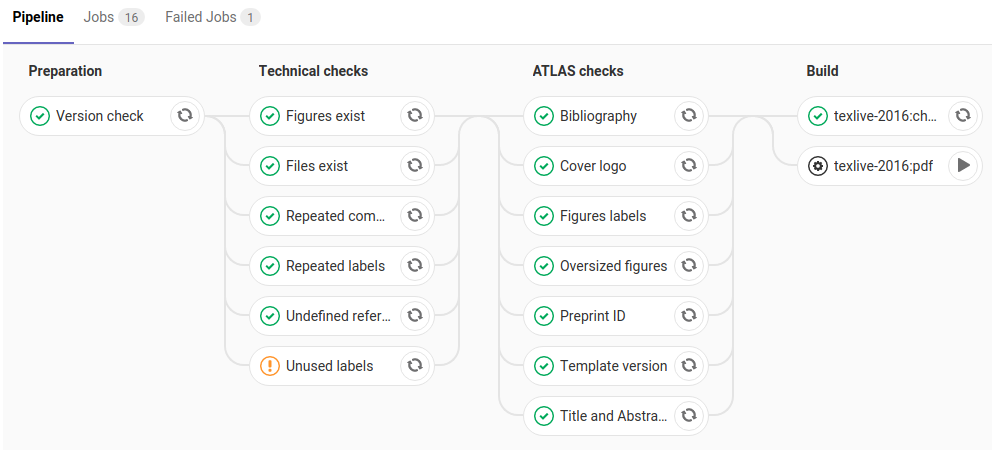
\includegraphics[width=0.9\textwidth]{edit-pipe.png}
  \caption{Screenshot of \epipe.}
  \label{fig:edit-pipe}
\end{figure}

\begin{table}
  \centering
  \begin{tabular}{l|c|c}
    \toprule
    \textbf{Document type} & \textbf{Preliminary label} & \textbf{Interl label} \\
    \midrule
    PAPER	& Not allowed	& Not allowed \\\midrule
    BOOK &	Not allowed	& Not allowed \\\midrule
    CONF &	Allowed	& Not allowed \\\midrule
    PUB &	Allowed	& Not allowed \\\midrule
    NOTE &	Allowed	& Allowed \\\bottomrule
  \end{tabular}
  \caption{Labels allowed and not allowed in figures depending on the document type.}
  \label{tab:labels-files}
\end{table}

%-------------------------------------------------------------------------------

%-------------------------------------------------------------------------------
% The PO GitLab area
\section{Physics Office Gitlab area}
\label{sec:pogitlab-group}
%-------------------------------------------------------------------------------

%-------------------------------------------------------------------------------
% Glance and GitLab integration
\section{The Analysis and Publications Glance interface}%Gabriela
\label{sec:anaglance}
Fence is a PHP framework designed after is was noticed that many of the Glance systems had similar features and the developers team turnover was big. Thus, the goal of the Fence project was to create a Web framework in which the Glance management systems could be developed in a way to favour the development of software requirements, reducing maintenance costs and speeding up the development process.

Fence was built using oriented object programming what made possible the creation of many classes that could be used among the Glance systems. One example is the GlanceSearch class allowing the creation of search interfaces with only some lines of code and the specification of the search attributes in a configuration file. The SuperSearch class provides an advanced search interface, where the user can build logic queries with AND and OR operators. The User class supports the access control of the interfaces. The Mailer class can be used in order to send emails from the interfaces. Form inputs can be easily added using the classes TextInput, to add text inputs, DateInput, to add date inputs, MemberInput, to add a selection box with a list of all the members of one experiment, and many others already implemented.

The Fence Workflow class is one more of the in the set that can be inherited by the systems using the framework. That can be used to program any process involving proceeding states and actions triggered while moving to a state do another. (explain better how it was built?)

For many years ATLAS has been using Glance to support the approval process of Papers, CONF and PUB notes. Since then they were considered independent systems, so they had different creation and search interfaces and also different workflows, all starting from its own Phase 1. As recently many projects at CERN changed their version control software from SVN to Gitlab, this has triggered the need of new Glance/Fence interface that could automatically create and configure Gitlab repositories. Thus, this new interface was created and called Phase 0.

The Phase 0 is common to Papers, CONF and PUB notes workflows, before Phase 1. It stores some metadata divided in steps, for example, meeting dates, comments and links, the groups of people there are Analysis Contact and their target date for Analysis finalisation, the groups of people there are Editorial board, approval sign-off dates and others. It also stores some basic metadata as short and full title, leading group, subgroups, Analysis Team members and supporting documents that will be after propagated to the publication (Paper, CONF note or PUB note) that proceeds Phase 0.

The Phase 0 system is where all the Gitlab environment for an ATLAS publication is set. When Phase 0 starts, a Gitab group is created to store one or more repositories related to the publication that should be written. A repository for one first internal document is also created with some template files and variables correctly substituted. The access control of those groups and repository are also set by the system, being the group of the Analysis Team defined in Phase 0. Also, some branches of the repositories are correctly created and protected.

In addition to the first internal document repository, more repositories can be created through Phase 0 system. One Phase 0 can have one or more internal document and one for a CONF note, PUB note or Paper. Detectors groups, those who need PUB notes or even Internal note for local reviews in sub-systems don’t have the necessity to go through the Phase 0 workflow, so they can to skip it and go directly to the Glance creation of a any type of publication, that, normally, happens at the end of Phase 0 workflow.

It can happen that a Phase 0 never evolves to become a Paper, CONF or PUB note, and turn into an internal document. In this case, the workflow will stop in Phase 0 and only internal documents repositories will exists. Also, if at any point the group convener decides that the Analysis should be discontinued, the deletion of the Phase 0 can be requested.

In some cases there is the need to create a Phase 0 entry very similar with one that already exists. The system allows that the existent entries can be cloned into new Phase 0 entries.

%-------------------------------------------------------------------------------

%-------------------------------------------------------------------------------
\section{The Physics Office Glance Gitlab integration}%all
\label{sec:poggintg}
%-------------------------------------------------------------------------------

%-------------------------------------------------------------------------------
\subsection{Author lists integration}%Gianluca,Maurizio,Gabriela
\label{sec:auth}

\begin{itemize}
\item Previous authorlist workflow:
AFS, script and problems.

\item New authorlist workflow:
Illustrating this new workflow, at Paper Phase 1, when an Authorlist is created a commit is done in Paper repository adding the first version of the Authorlist files in all available formats. At Phase 2, if the Authorlist has a new change, like a new exception, a new commit will be done, substituting the previous version of the Authorlist files.
In summary: Gitlab will store the last updated version of the Authorlist files.
Similarly to the interface used nowadays on the Web, Glance has an interface listing all author list already created in all available formats. The difference with the old Web is that some will point to AFS (old archived author lists) and some will point to Gitlab (newly generated author lists through Glance).
Tickets:
https://its.cern.ch/jira/browse/ATGLANCE-1997
https://its.cern.ch/jira/browse/ATGLANCE-1996
https://its.cern.ch/jira/browse/ATGLANCE-1990
https://its.cern.ch/jira/browse/ATGLANCE-1987
https://its.cern.ch/jira/browse/ATGLANCE-1912
https://its.cern.ch/jira/browse/ATGLANCE-1911
https://its.cern.ch/jira/browse/ATGLANCE-1910
https://its.cern.ch/jira/browse/ATGLANCE-1908

Minutes from POGG meeting can help. The email was sent by Fairouz with subject "POGG minutes"
\end{itemize}

%-------------------------------------------------------------------------------

% All figures and tables should appear before the summary and conclusion.
% The package placeins provides the macro \FloatBarrier to achieve this.
% \FloatBarrier

%-------------------------------------------------------------------------------
\section{Conclusion}
\label{sec:conclusion}
%-------------------------------------------------------------------------------

Place your conclusion here.


%-------------------------------------------------------------------------------
% Bibliography
\printbibliography
%-------------------------------------------------------------------------------

%-------------------------------------------------------------------------------
\clearpage
\appendix
\part*{Appendices}
\addcontentsline{toc}{part}{Appendices}
%-------------------------------------------------------------------------------

In an ATLAS note, use the appendices to include all the technical details of your work
that are relevant for the ATLAS Collaboration only (e.g.\ dataset details, software release used).
This information should be printed after the Bibliography.

\end{document}
